\documentclass[12pt, letterpaper, spanish, twoside]{article}
\AddToHook{cmd/section/before}{\newpage}
\usepackage{./common/UAQ}

\graphicspath{{./figures/}}

\begin{document}

% Fondo de portada
\backgroundsetup{
	scale = 1,
	angle = 0,
	opacity = 1,
	contents = {
		
\includegraphics[width=\paperwidth]{CoverBackground.pdf}
	}
}

\begin{titlepage}

\vspace*{10cm}
{\huge \bfseries \textcolor{RojoUAQ}{Plantilla para protocolo de tesis de maestría de la Facultad de Ingeniería, Universidad Autónoma de Querétado}\\[1cm] }

\begin{center}
	\noindent
	\begin{minipage}{0.4\textwidth}
	\begin{flushleft} \large
	\emph{Estudiante:}\\
	Ing. Arya Stark
	\end{flushleft}
	\end{minipage}	
	\begin{minipage}{0.4\textwidth}
	\begin{flushright} \large
	\emph{Director:} \\
	Dr. Syrio Forel \\[1.5cm]
	\emph{Codirector:} \\
	Dr. Jaqen H'ghar
	\end{flushright}
	\end{minipage}
    
	\vfill
    
	{\large \today}
\end{center}
\end{titlepage}


\backgroundsetup{
	scale = 1,
	angle = 0,
	opacity = 1,
	contents = {
		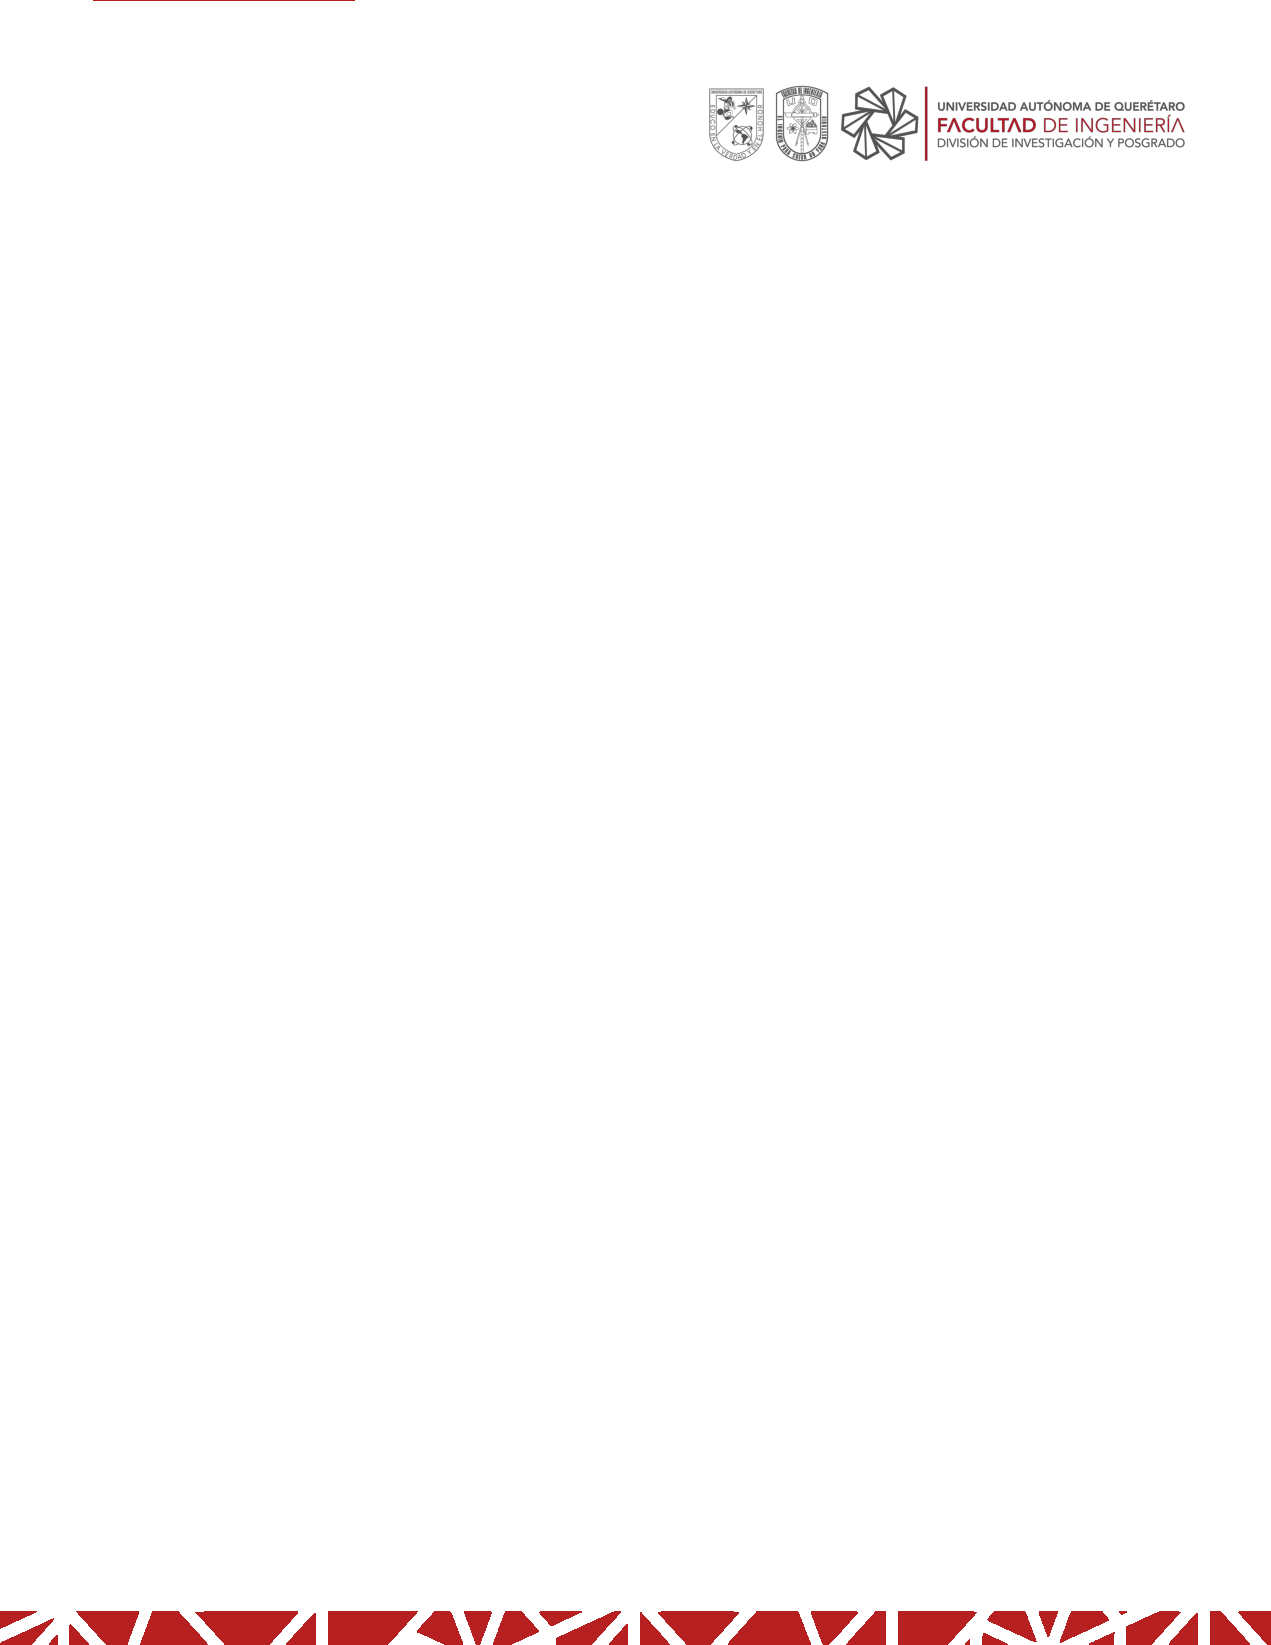
\includegraphics[width=\paperwidth]{BodyBackground.pdf}
	}
}

\pagenumbering{roman}
\tableofcontents

\pagenumbering{arabic}
\section*{Datos generales}
\addcontentsline{toc}{section}{Datos generales}
\begin{itemize}
	\item Título del proyecto de Tesis
	\item Nombre del alumno
	\item Número de expediente
	\item Programa de Estudios a realizar (maestría o doctorado)
	\item Director de Tesis
	\item Secretario
	\item Vocal
	\item Lugar donde se realizará la investigación
	\item Línea de investigación
	\item Tipo de investigación [básica, aplicada o tecnológica (diseño, construcción de prototipo o prueba experimental)]
	\item Horario de trabajo:
\end{itemize}

\section{Resumen}
Lorem ipsum dolor sit amet, consectetur adipiscing elit. Donec semper, orci at commodo pharetra, eros nisi iaculis mauris, et vehicula metus arcu eget ex. Phasellus at magna nec ex sodales consectetur. Duis nisl sem, mattis nec euismod in, viverra in nibh. Sed nibh metus, consequat eget rhoncus ac, feugiat vel libero. Curabitur blandit, ante sit amet fringilla interdum, ex mauris pharetra enim, id semper mi diam sit amet erat. Aliquam elementum ultricies turpis, et volutpat tortor dignissim consectetur. Vivamus auctor ex ut dolor luctus consectetur. Sed vel nisi sit amet augue rhoncus dignissim eget ut est. Nulla in leo varius, facilisis ex ac, fringilla orci. Curabitur placerat tincidunt commodo.


\section{Antecedentes}
Los antecedentes describen la evaluación actual.

\section{Justificación}
Consiste en la exposición de motivos o razones para la investigación. 

\section{Descripción del problema}
Se identifican los fenómenos, hechos o situaciones, que puestos en relación presentan incongruencias, obstáculos, desconocimiento o discrepancia y que constituyen el objeto.

\section{Fundamentación teórica}
Se refiere al planteamiento del sustento teórico que constituye la base para solucionar los problemas planteados. La Fundamentación Teórica consiste en el planteamiento de:

\begin{enumerate}
	\item La perspectiva desde donde se desarrollará el estudio (modelo teórico, básico).
	\item Los elementos del tema que se consideran más significativos (variables con las cuales va a interactuar el investigador).
	\item Los instrumentos teóricos de análisis de los datos obtenidos.
\end{enumerate}


\section{Hipótesis}
La hipótesis es un enunciado a renglón corrido, que plantea una posible respuesta a la pregunta de investigación basada en la teoría y en la práctica, estableciendo relaciones entre las variables del problema y que al contrastarse proporcionará conocimiento nuevo en la diciplina de estudio.

\begin{enumerate}
	\item Variables de entrada (unidad de análisis)
	\item Variables de salida (unidad de análisis)
	\item Fundamento teórico y/o práctico
	\item Relaciones entre variables de entrada y variables de salida.
	\item Supuesto(s)
	\item Redactar la hipótesis, con lo ingresado en los campos anteriores.
\end{enumerate}


\section{Objetivos}
Los objetivos son los propósitos del trabajo de investigación y relacionan los entregables con la metodología de la investigación. Deben ser específicos, medibles, alcanzables, orientados a resultados y deben esta definidos en el tiempo.

\begin{enumerate}
	\item Objetivo general 
	\item Objetivos específicos 
	\item Cronograma de actividades 
\end{enumerate}


\section{Metodología}
Descripción detallada de los procedimientos y las técnicas a utilizar para la obtención de los datos y el proceso de los mismo; especificando los materiales, las herramientas y los métodos que se usarán para verificar la hipótesis y lograr los objetivos del trabajo de investigación, a un nivel de detalle suficiente que permita la réplica del trabajo.


\section{Recursos}
Se deben describir los recursos que se usan en la investigación:

\begin{enumerate}
	\item Maquinaría:
	\begin{itemize}
		\item Nombre.
		\item Describir brevemente el uso adecuado de cada máquina incluyendo, si es necesario, las medidas de seguridad necesarias para su manejo.
		\item Describir el manejo de los deshechos y/o residuos.
	\end{itemize}

	\item Equipos:
	\begin{itemize}
		\item Nombre.
		\item Describir brevemente el uso adecuado de cada equipo incluyendo, si es necesario, las medidas de seguridad necesarias para su manejo.
		\item Describir el manejo de los deshechos y/o residuos.
	\end{itemize}

	\item Químicos de laboratorio:
	\begin{itemize}
		\item Nombre de reactivo.
		\item Indicar los aspectos de buenas prácticas de laboratorio, para el uso del reactivo, con los que se capacitará al equipo de trabajo.
		\item Establecer la disposición de los residuos al término de la experimentación y las medidas de seguridad consideradas para su trazabilidad.
		\item Anexar documentos que autoricen el uso del recurso.
	\end{itemize}
	
	\item Biológicos:
	\begin{itemize}
		\item Nombre del recurso biológico.
		\item Indicar los aspectos de buenas prácticas de laboratorio, para el uso del recurso biológico, con los que se capacitará al equipo de trabajo.
		\item Establecer la disposición de los residuos al término de la experimentación y las medidas de seguridad consideradas para su trazabilidad.
		\item Indicar el origen del recurso biológico. 
		\item Anexar documentos que autoricen el uso del recurso.
	\end{itemize}
	
	\item Renovables:
	\begin{itemize}
		\item Flora
		\begin{itemize}
			\item Nombre de la especie de flora.
			\item Describir las buenas prácticas del manejo del recurso que apliquen a la investigación, considerando manuales, procedimiento y/o normas nacionales o internacionales.
			\item Establecer la disposición de los residuos al término de la experimentación y las medidas de seguridad consideradas para su trazabilidad.
			\item Anexar documentos que autoricen el uso del recurso.
		\end{itemize}
		
		\item Fauna
		\begin{itemize}
			\item Nombre de la especie de fauna.
			\item Describir las buenas prácticas del manejo del recurso que apliquen a la investigación, considerando manuales, procedimiento y/o normas nacionales o internacionales.
			\item Establecer la disposición de los residuos al término de la experimentación y las medidas de seguridad consideradas para su trazabilidad.
			\item Anexar documentos que autoricen el uso del recurso.
		\end{itemize}			
		
		\item Agua
		\begin{itemize}
			\item Indicar la categoría de su clasificación.
			\item Describir brevemente su fuente.
			\item Establecer la disposición de los residuos.
			\item Anexar documentos que autoricen el uso del recurso.
		\end{itemize}
		
		\item Suelos
		\begin{itemize}
			\item Nombre del tipo de suelo.
			\item Descripción breve del tipo de suelo y el origen.
			\item Establecer la disposición de los residuos.
			\item Anexar documentos que autoricen el uso del recurso.
		\end{itemize}
		
		\item Otros
		\begin{itemize}
			\item Nombre de recurso.
			\item Descripción breve del recurso.
			\item Describir brevemente su fuente.
		\end{itemize}
	\end{itemize}
	
	\item No renovables:
	\begin{itemize}
		\item Metálicos
		\begin{itemize}
			\item Nombre de recurso.
			\item Descripción breve del recurso.
			\item Describir brevemente su fuente.
		\end{itemize}
		
		\item No metálicos
		\begin{itemize}
			\item Nombre de recurso.
			\item Descripción breve del recurso.
			\item Describir brevemente su fuente.
		\end{itemize}
		
		\item Combustibles fósiles
		\begin{itemize}
			\item Nombre de recurso.
			\item Descripción breve del recurso.
			\item Describir brevemente su fuente.
		\end{itemize}
		
		\item Radioactivos
		\begin{itemize}
			\item Nombre de recurso.
			\item Descripción breve del recurso.
			\item Describir brevemente su fuente.
		\end{itemize}
		
		\item Otros
		\begin{itemize}
			\item Nombre de recurso.
			\item Descripción breve del recurso.
			\item Describir brevemente su fuente.
		\end{itemize}
	\end{itemize}
	
	\item Materiales nanoestructúrales:
	\begin{itemize}
		\item Nombre.
		\item Descripción breve del material.
		\item Procedimientos de seguridad en su uso y manipulación.
		\item Describir el manejo de los deshechos y/o residuos, si es que lo hay.
		\item Anexar documentos que autoricen el uso del recurso.
	\end{itemize}
	
	\item Información:
	\begin{itemize}
		\item ¿La información implementada ya existe en alguna base de datos? SI/NO
		\begin{itemize}
			\item Descripción breve de qué tipo de información se utilizará para la investigación.
			\item ¿La información pertenece a una institución o empresa del sector privado? SI/NO
			\begin{enumerate}
				\item Describe y adjunta la siguiente documentación: 
				\begin{enumerate}
					\item Formato de solicitud de información.
					\item Permisos de uso de información.
				\end{enumerate}
			\end{enumerate}
		\end{itemize}
		
		\item ¿Su investigación requiere de información obtenida de seres humanos como fuente de información? SI/NO
		\begin{itemize}
			\item Realiza una descripción.
			\item Indica cuales son los criterios de inclusión y exclusión que se implementaron para la selección de los participantes.
			\item Anexa documento de consentimiento informado.
			\item ¿La investigación discrimina la participación de las / los individuos, o incluye un trato diferenciado entre las / los participantes, con base a su género, raza o grupo étnico, edad, religión, ingreso económico, desventaja o discapacidad, enfermedad o cualquier clasificación similar? (Sí es SI, describe el motivo).
			\item ¿La investigación incluye la participación de individuos socialmente o físicamente vulnerables (hombres y mujeres menores de edad, adultos mayores, con capacidades diferentes, etc) o los grupos legalmente restringidos o aislados, o el uso inadecuado de la información puede Confidencial 03/12/2018 Manual de procedimientos DOCUMENTADOS. 4 afectar en algún sentido la integridad de los individuos? (Sí es SI, describe).
		\end{itemize}
	\end{itemize}

\end{enumerate}


\section{Alcance del proyecto}
Impacto, proyección y trascendencia de la investigación, ya sea de tipo científico, tecnológico, económico, cultural o social. Determinación de qué elementos del proyecto se incluyen o no en la investigación y sus razones. Debe dimensionar y delimitar la investigación considerando los resultados, el impacto, la calidad, tiempo y recursos económicos prospectados.


\section{Resultados esperados}
Se especifican los productos del trabajo, su impacto científico, tecnológico y económico.

\nocite{*} % Para mostrar todas las refencias sin citarlas
\renewcommand{\refname}{Referencias bibliográficas}
\bibliographystyle{IEEEtran}
\bibliography{referencias}

\end{document}